\documentclass[tikz,border=2pt]{standalone}
\usepackage{tikz}
\usetikzlibrary{calc}

\begin{document}
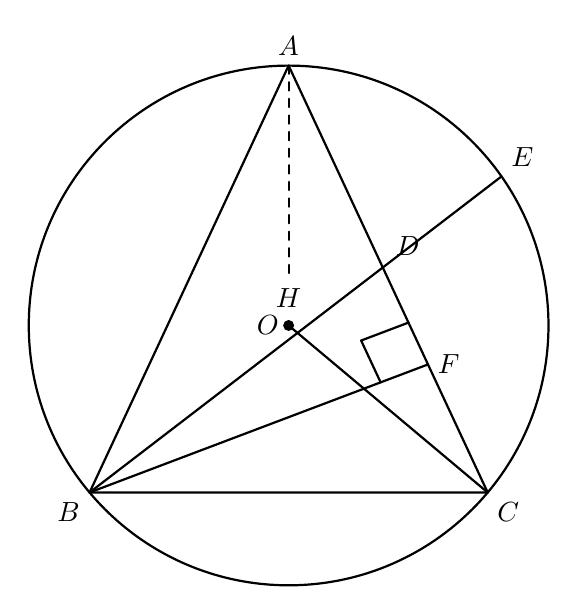
\begin{tikzpicture}[scale=1.1, line cap=round, line join=round]

% Coordinates
\def\R{3}
\coordinate (O) at (0,0);
\coordinate (A) at (90:\R);
\coordinate (B) at (220:\R);
\coordinate (C) at (320:\R);
\coordinate (H) at ($(A)!0.82!(O)$);

% Point E on circle and D on line BE
\coordinate (E) at (35:\R);
\coordinate (D) at ($(B)!0.72!(E)$);

% Point F on AC and segment BF perpendicular-ish to AC
\coordinate (F) at ($(A)!0.70!(C)$);

% Circle
\draw[thick] (O) circle (\R);

% Triangle and other segments
\draw[thick] (A)--(B)--(C)--cycle;
\draw[thick] (B)--(F);
\draw[thick] (O)--(C);
\draw[thick] (B)--(D); % keep part of line BE up to D
\draw[thick] (D)--(E); % keep part from D to E
\draw[dashed, thick] (A)--(H);

% Right angle mark near F between AC and BF
\coordinate (r1) at ($(F)!0.14!(A)$);
\coordinate (r2) at ($(F)!0.14!(B)$);
\coordinate (r3) at ($(r1)+(r2)-(F)$);
\draw[thick] (r1)--(r3)--(r2);

% Points
\fill (O) circle (1.8pt);

% Labels
\node[above] at (A) {$A$};
\node[below left] at (B) {$B$};
\node[below right] at (C) {$C$};
\node[above right] at (E) {$E$};
\node[above right] at (D) {$D$};
\node[right] at (F) {$F$};
\node[left] at (O) {$O$};
\node[below] at (H) {$H$};

\end{tikzpicture}
\end{document}
